\lstnewenvironment{jastaddcode}
	{\lstset{
		basicstyle=\footnotesize\ttfamily,
		keywordstyle=\ttfamily\bfseries,
		commentstyle=\itshape\sffamily,
		tabsize=4,
		xleftmargin=0.2cm, %\parindent
		basewidth=0.6em,
		fontadjust= true,
		lineskip=0.7pt,
		aboveskip=\baselineskip,
		belowskip=\baselineskip,
		frame=tb,
		showspaces=false,
		showtabs=false,
		framerule=0.5pt,
		framexleftmargin=0.2cm,
		numbers=none,
		}
	}
	{}

\section{JastAdd}

%
% Introduction
%
\subsection{Introduction}
The JastAdd metacompilation tool~\cite{magnusson03scp} builds on object-oriented concepts: The abstract grammar is represented as a class hierarchy, and the abstract syntax tree (AST) as a tree of objects of those classes. The JastAdd specification formalism makes use of \emph{reference attributed grammars}~\cite{hedin00informatica} (RAGs), which extends Knuth's attribute grammars~\cite{knuth68mst}: An attribute is allowed to be a \emph{reference} to another node in the AST, and attributes in that node can be remotely accessed via the reference. For example, an Oberon-0 identifier has a reference attribute \texttt{decl} that points to the declaration of the identifier, and the identifier can find its type simply by remotely accessing the \texttt{type} attribute of its declaration, see Figure \ref{JA-UseDecl}.

A JastAdd specification declares a number of abstract grammar classes, attributes in such classes, and equations defining the values of those attributes. The specification is declarative in the sense that in an evaluated AST, the attributes will have values such that the equations hold. The order of evaluation is given implicitly, by the attribute dependencies in the equations, and evaluation is performed on demand \cite{jourdan84isp}. This declarative system can be integrated with imperative code that may read (but not write) attribute values. For example, the Oberon-0 code generator is implemented as methods that traverse the AST and output code to a file, reading attributes to decide what code to output. The AST is constructed by a parser, and attribute evaluation is then performed automatically, on demand, as attribute values are read.

A key feature of JastAdd is its modularity, allowing language constructs and computations to be modularized and extended. This is supported by the declarative computations (e.g., the order of equations is insignificant), the object-oriented foundation (e.g., classes can be extended through subclassing, and equations can be overridden in subclasses), and the use of inter-type declarations like in AspectJ \cite{kiczales01ecoop} (e.g., attributes of a class can be declared syntactically outside of the class).
For the Oberon-0 compiler, this is used to modularize the compiler according to the different artifacts, and the subproblems in those artifacts.

The JastAdd tool supports several kinds of attributes, and the ones used in the Oberon-0 compiler are summarized in Figure~\ref{JA-AttributeKinds}.

\begin{figure}
\begin{center}
\begin{tabular}{ | l c | l | l | }
  \hline             
  \multicolumn{2}{|l|}{\bf{attribute kind}} & \bf{description} & \bf{example use} \\
  \hline
  \hline          
  \emph{synthesized}& \multirow{2}{*}{\cite{knuth68mst}} & defined in the node & actual type \\
  \emph{inherited}& & defined in a parent node & expected type \\
  \hline 
  \emph{reference}& \multirow{2}{*}{\cite{hedin00informatica}}& can point to AST node & \multirow{2}{*}{name lookup}\\
  \emph{parameterized}& & can have argument & \\
  \hline
  \emph{non-terminal}& \cite{vogt89pldi}& a fresh AST subtree & predefined declaration \\
  \hline
  \emph{collection}& \cite{boyland98cc,magnusson09ase}& defined by set of partial values & compile-time errors \\
  \hline  
\end{tabular}
\caption{Attribute kinds used in the JastAdd Oberon-0 compiler.}
\label{JA-AttributeKinds}
\end{center}
\end{figure}


%
% Architecture and Parsing
%
\subsection{Architecture and Parsing}
A JastAdd specification consists a number of files with extensions \texttt{.ast} (abstract grammar), \texttt{.jrag} (attributes and their equations), and \texttt{.jadd} (imperative methods). The JastAdd tool is fed a number of these files as input, and produces Java source code as output. In this process, Java classes are generated corresponding to the abstract grammar in the \texttt{.ast} files, and code is woven into these classes, corresponding to the attributes, equations, and methods in the \texttt{.jrag} and \texttt{.jadd} files.

Scanning and parsing can be done with any tools that can create arbitrary Java objects as a result of the parse. For Oberon-0, the \emph{JFlex} scanner generator and the \emph{Beaver} parser generator are used, and code is added to the semantic actions of Beaver, to create ASTs according to the JastAdd abstract grammar.

To complete the compiler, a main program needs to be written in Java. The main program calls the parser to build the AST, and then produces some output based on the attributed AST, e.g., by calling a code generation method. Note that the main program does not need to invoke any evaluation code: as soon as the AST is built, its attributes can be accessed, since they are evaluated on demand. Figure~\ref{JA-GenerationProcess} shows a typical compiler generation process.

\begin{figure}[h]
\begin{center}
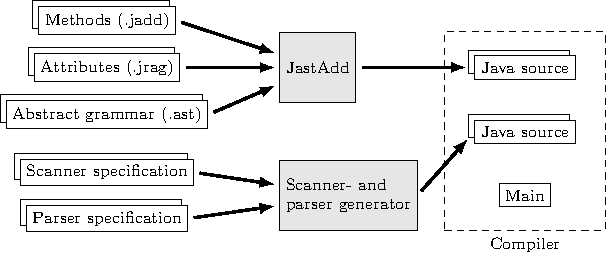
\includegraphics{jastadd/generation-process.pdf}
\caption{A typical compiler generation process using JastAdd.}
\label{JA-GenerationProcess}
\end{center}
\end{figure}

For the Oberon-0 compiler, the artifacts are specified in different directories: \texttt{A1}, \texttt{A2a}, \texttt{A2b}, \texttt{A3}, and \texttt{A4}. Within each directory, there are specification files for scanner, parser, abstract grammar, attributes, and methods. Typically, there are several attributes and methods files for different subproblems, e.g., name analysis, type checking, etc. Each artifact (except for \texttt{A1}) extends one or more previous artifacts, and its directory contains the specification files for that extension only. To build an artifact, an \emph{Ant} build file is used that simply lists all the relevant specification directories. This allows reuse of all the specification files from the previous artifacts, and only the build script and the main program need to be written specifically for the artifact. An explicit import mechanism would have been preferable to simply listing directories in the build script, but this is currently lacking in JastAdd. Figure~\ref{JA-ArtifactsOverview} shows all the specification files in the different artifact directories, their size, and how they depend on each other.

\begin{figure}[h]
\begin{center}
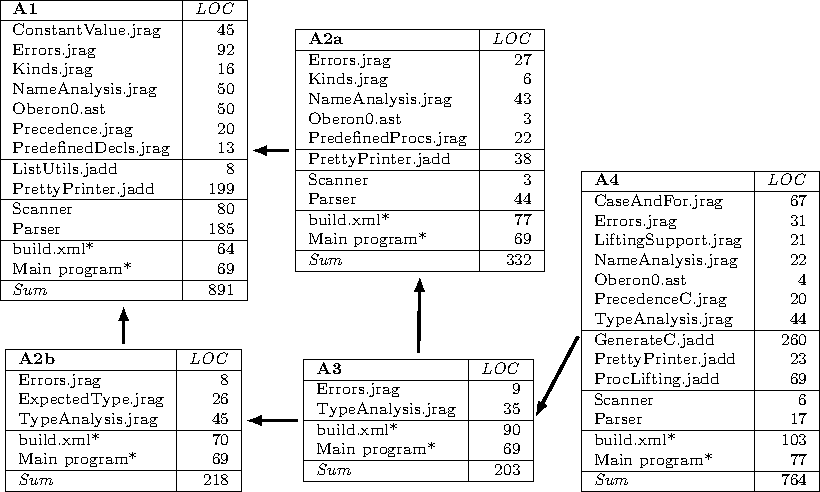
\includegraphics{jastadd/artifacts-overview.pdf}
\caption{An overview of modules in artifacts and how they extend each other. Arrow means extension and * means that the file is not reused.}
\label{JA-ArtifactsOverview}
\end{center}
\end{figure}

Figure~\ref{JA-AbsGram} shows some of the abstract grammar classes defined in the \texttt{A1} artifact. Abstract grammars are typically extended by adding new subclasses. For example, to extend Oberon-0 with procedures, a new class \texttt{Procedure} is defined in the \texttt{A2a} artifact, as a subclass of \texttt{Decl}.

\begin{figure}[h]\footnotesize
\begin{jastaddcode}
Module ::= <StartId> Decl* Block <EndId>; // The root class
abstract Decl;                     // Superclass for declarations
abstract Stmt;                     // Superclass for statements
Block : Stmt ::= Stmt*;            // Subclass for blocks
abstract Expr;                     // Superclass for expressions
abstract Access : Expr;            // Subclass for accesses
SimpleAccess : Access ::= IdUse;   // Subclass for access to simple var
IdDecl ::= <ID>;                   // Declared identifier
IdUse ::= <ID>;                    // Use of a declared identifier
...
\end{jastaddcode}
\vspace{-15pt}
\caption{Some of the abstract grammar classes defined in \texttt{A1/Oberon0.ast}. Tokens are enclosed in angle brackets. Lists are indicated by the Kleene star.}
\label{JA-AbsGram}
\end{figure}

Unfortunately, JFlex and Beaver do not support modularized specifications. For JFlex, we currently use a workaround by splitting the specification into several files, and concatenating them in different ways in the different build scripts. For Beaver, we use a preprocessor, called \emph{JastAddParser}, that has a specification similar to Beaver's, but where different productions can be specified in different files. This allows us to achieve the desired modularization also for the parsing, although in a somewhat clumsy way.


%
% Name analysis
%
\subsection{Name analysis}
\label{JA-NameAnalysis}
The task of name analysis is to bind an identifier usage to the corresponding declaration,
taking into account the language's scope rules. For Oberon-0, we represent identifier usages by the class \texttt{IdUse}, declarations by \texttt{IdDecl}, and bindings by a reference attribute \texttt{decl} in \texttt{IdUse}. The \texttt{decl }attribute is defined using an inherited parameterized attribute \texttt{lookup(String)}. This attribute is defined in some parent of the \texttt{IdUse}, typically in a procedure or a module, and will find the appropriate \texttt{IdDecl} node, given the identifier name as argument. This design makes it unnecessary to construct explicit symbol tables or environment data structures: we can instead use the AST itself as this structure. The Figure~\ref{JA-DeclNameAnalysis} shows part of the name analysis for artifact \texttt{A1}, and an example is shown in Figure~\ref{JA-UseDecl}. The equation in \texttt{Module} makes use of two other parameterized attributes, \texttt{localDeclLookup} and \texttt{localPredefinedLookup}, to delegate the search to the local declarations and the predefined declarations, respectively.

\begin{figure}
\begin{jastaddcode}
syn IdDecl IdUse.decl() = lookup(getID());
inh IdDecl IdUse.lookup(String name);
eq Module.getBlock().lookup(String name) {
    IdDecl decl = localDeclLookup(getNumDecl()-1, name);
    if (decl == null) decl = localPredefinedLookup(name);
    return decl;
}
\end{jastaddcode}
\vspace{-15pt}
\caption{Part of the name analysis for Oberon-0}
\label{JA-DeclNameAnalysis}
\end{figure}

\begin{figure}[h]
\begin{center}
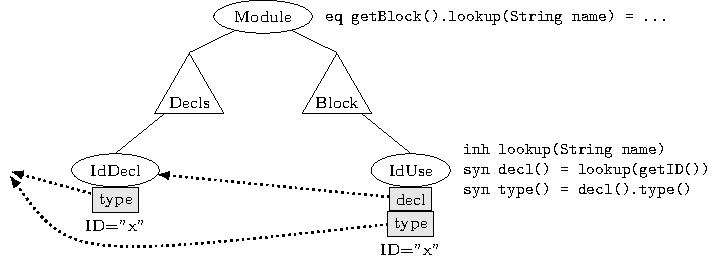
\includegraphics{jastadd/use-decl.pdf}
\caption{An AST illustrating how uses are bound to declarations, with the \texttt{decl} attribute. 
	Ellipses are AST nodes. Triangles are subtrees. Rectangles are attributes. 
	Solid lines are child/parent links. Dotted lines are reference values.}
\label{JA-UseDecl}
\end{center}
\end{figure}

In artifact \texttt{A2a}, procedures are added, and the name analysis needs to be extended with support for nested scopes. The Figure~\ref{JA-ProcNameAnalysis} shows how this is handled: The abstract syntax is extended with classes for \texttt{Procedure} and \texttt{ProcedureCallStmt}, and an equation for \texttt{lookup} is added in \texttt{Procedure}. The equation first searches locally among parameters and declarations in the procedure, and if no match is found there, the search is delegated to the context of the \texttt{Procedure}, using the l\texttt{ookup} attribute of the \texttt{Procedure} itself. This attribute is also declared in the figure, and will be defined by a parent \texttt{Module} or \texttt{Procedure} node, depending on the structure of the program.

\begin{figure}
\begin{jastaddcode}
Procedure : Decl ::= IdDecl ParDecl* Decl* Block <EndId>;
ProcedureCallStmt : Stmt ::= IdUse Expr*;

eq Procedure.getDecl(int index).lookup(String name) {
	IdDecl decl = localParLookup(name);
	if (decl == null) decl = localDeclLookup(index, name);
	if (decl == null) decl = lookup(name);
	return decl;
}
inh IdDecl Procedure.lookup(String name);
\end{jastaddcode}
\vspace{-15pt}
\caption{Extending Oberon-0 with procedures and nested name analysis} 
\label{JA-ProcNameAnalysis}
\end{figure}

In Oberon-0, constants, types, variables and procedures all use the same namespace. 
We can therefore use \texttt{IdDecl} and \texttt{IdUse} for all these
constructs, and share the definition of the \texttt{lookup} attribute between them.
To handle the \emph{declare before use} policy that applies within a declaration part, for example to look up type names, an additional parameter is used for \texttt{localDeclLookup}, to search only up to a certain point in the declaration list.

Oberon-0 contains a number of predefined declarations, e.g., the types \texttt{INTEGER} and \texttt{BOOLEAN}. In order to allow these to be handled in the same way as user-defined declarations, they are also represented in the AST. This is done using the NTA \texttt{predefinedDecls} in \texttt{Module}. A \emph{non-terminal attribute} (NTA) is both an attribute and an AST subtree at the same time, and is also called a \emph{higher-order attribute}~\cite{vogt89pldi}. The subtree of an NTA is created as the result of evaluating its defining equation. Figure~\ref{JA-PredefinedDecls} shows how a variable declaration uses the predefined type \texttt{INTEGER}, and how the \texttt{IdUse} of its type is bound to the \texttt{IdDecl} declaring \texttt{INTEGER} in the NTA.


%
% Type checking
%
\subsection{Type checking}
\label{JA-TypeChecking}

To typecheck an Oberon-0 expression, we compare its actual type with the type expected by its context. This is captured in two attributes: the inherited attribute \texttt{expectedType} and the synthesized attribute \texttt{type}. For example, for an assignment, the expected type of the right-hand side expression is the same as the type of the left-hand side variable, see Figure~\ref{JA-ExpectedType}.

\begin{figure}[h]
\begin{jastaddcode}
inh Type Expr.expectedType();

eq AssignmentStmt.getExpr().expectedType() = getAccess().type();
eq IfStmt.getExpr().expectedType() = module().boolType();
...
\end{jastaddcode}
\vspace{-15pt}
\caption{Definition of the inherited attribute \texttt{expectedType}}
\label{JA-ExpectedType}
\end{figure}

Type-checking errors, and other compile-time errors, are collected into a set-valued attribute \texttt{errors} in the \texttt{Module} node (the root of the AST). The \texttt{errors} attribute is a \emph{collection attribute}  \cite{boyland98cc,magnusson09ase} whose value is defined by \emph{contribution} rules, one for each possible compile-time error. 
Figure~\ref{JA-TypeErrors} shows how type-checking errors are collected, simply by contributing an error object when the actual and expected types are not compatible. Here, \texttt{error(String s)} is a method returning a fresh error object, \texttt{compatibleWith(Type~t)} is a parameterized synthesized attribute for comparing types, and \texttt{module()} is an inherited attribute returning the \texttt{Module} root node.

\begin{figure}[h]
\begin{jastaddcode}
Expr contributes error("Type error ...")
	when !type().compatibleWith(expectedType())
	to Module.errors() for module();
\end{jastaddcode}
\vspace{-15pt}
\caption{Collection of type checking errors}
\label{JA-TypeErrors}
\end{figure}

The synthesized attribute \texttt{type} is defined for the different kinds of expressions. For operators, the value is typically a predefined type, like \texttt{INTEGER} or \texttt{BOOLEAN}. The type of a variable or constant access is normally the type of its declaration. However, we also need to take into account that the declaration may be missing, or it may be a circularly defined constant, like \texttt{CONST c = c}. In these cases, we represent the type by an object \texttt{unknownType}, see Figure~\ref{JA-SimpleIdUse}. 

\begin{figure}
\begin{jastaddcode}
syn Type Expr.type();
eq RelationExpr.type() = module().boolType();
eq ArithmeticBinExpr.type() = module().integerType();
...
eq SimpleAccess.type() = getIdUse().type();

syn Type IdUse.type() {
	if (decl() == null || isCircular()) 
		return module().unknownType();
	return decl().type();
}
\end{jastaddcode}
\vspace{-15pt}
\caption{Definition of the synthesized attribute \texttt{type}}
\label{JA-SimpleIdUse}
\end{figure}

To resolve the type of a declaration, each \texttt{IdDecl} has an inherited attribute \texttt{type}. (Figure~\ref{JA-SimpleIdUse} showed an example use of the attribute.) Often, the type in a declaration is itself a use of a type declared elsewhere. It is then represented by a \texttt{TypeUse} node that contains an \texttt{IdUse} node which handles the name binding to the (type) declaration, just like for variables and constants. Figure~\ref{JA-PredefinedDecls} shows an example for the variable declaration \texttt{VAR~x~:~INTEGER;} The actual type of \texttt{x} is found by following the \texttt{decl} reference attribute in the type use. In this case, the type is located among the predefined declarations, in the NTA in the AST root.

\begin{figure}
\begin{center}
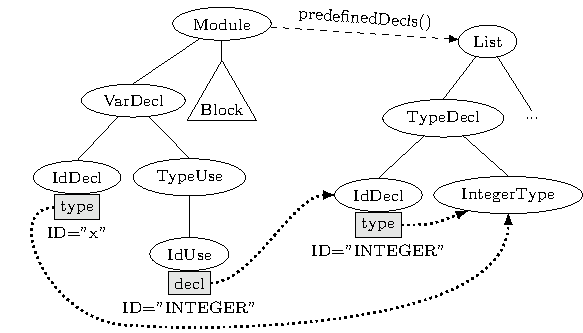
\includegraphics{jastadd/predefined-decls.pdf}
\caption{Shows binding of a type use, for \texttt{VAR x:INTEGER}, where \texttt{INTEGER} is a predefined type. Dashed lines are NTAs (e.g. \texttt{predefinedDecls}).}
\label{JA-PredefinedDecls}
\end{center}
\end{figure}


%
% Source-to-source transformation
%
\subsection{Source-to-source transformation}
Our implementation includes two kinds of source-to-source transformations: 1) procedure lifting in order to simplify generation of C code (since C functions cannot be nested), and 2) translating a larger language to a syntactically smaller core language, also to simplify code generation. 

Procedure lifting is implemented by generating a new AST where declarations of procedures, types and constants are moved to the top level. This is implemented as a method that traverses the original AST to build the new one, and uses attributes to decide what to build. For example, to generate new identifiers, the path from the root down to a declaration is used, and is captured by an inherited attribute \texttt{astPath} in \texttt{IdDecl}. The transformation is idempotent: applying the transformation more than once yields the same result. This is accomplished by using attributes to check if the original AST includes only top-level constructs.

To translate from a larger to a syntactically smaller language, NTAs are used. An example is translating \texttt{CASE} to \texttt{IF}.
This is done by defining an NTA \texttt{ifEquivalent} in \texttt{CaseStmt}. This simplifies code generation, since code can be generated for \texttt{CaseStmt} simply by delegating to the NTA. However, the NTA is only used for code generation: all compile-time error checking is still done directly in the original \texttt{CaseStmt}, in order to give error messages in terms of the original construct. The same technique is used to translate \texttt{FOR} to \texttt{WHILE}. Here, construction of the NTA is actually not simpler than just generating the code directly, but will pay off if several code generators for different targets are implemented.

%
% Code generation
%
\subsection{Code generation}
Generation of C code is implemented with a method \texttt{generateC}
that traverses the AST, making use of attributes to generate the correct code.
The code generation is similar to pretty printing, but needs to handle some additional things, like name collision with C's keywords, and that type declarations in C are structured in a somewhat different way. Parentheses are not stored in the AST, but are added during code generation and pretty printing, using attributes to encode the precedence rules.

To generate code for \texttt{CASE} and \texttt{FOR} is easy, it just amounts to delegating the work to the NTA. For example, the \texttt{ForStmt} class, delegates the code generation to its NTA \texttt{whileEquivalent}: 

\begin{jastaddcode}
public void ForStmt.generateC(StringBuilder sb, int indent) {
	whileEquivalent().generateC(sb, indent);
}
\end{jastaddcode}


%
%  Concluding observations
%
\subsection{Concluding observations}
\emph{Ease of use.} 
The main characteristic of JastAdd is its declarative specification technique that makes use of and blends with object-oriented programming: the AST is represented by an object-oriented model that arguably a normal OOP programmer would have constructed, but replaces imperative compiler phases with declarative computations in the form of attributes and equations.

In constructing the Oberon-0 compiler, we have reused a number of design ideas from earlier JastAdd compilers. These include:
\begin{itemize}
  \item Synthesized reference attributes, typically called \texttt{decl}, and inherited parameterized attributes, typically called \texttt{lookup}, for name analysis.
  \item Parameterized attributes that use double dispatch (calling another attribute) for comparing types~\cite{ekman07oopsla}.
  \item Collection attributes for collecting compile-time error messages.
  \item Non-terminal attributes for representing predefined declarations.
  \item Non-terminal attributes for representing new language constructs in terms of existing ones, in order to simplify code generation.
  \item Imperative methods that access attributes in order to implement pretty-printing and code generation.
\end{itemize}
We consider these design choices to be useful for most compiler implementations in JastAdd, and to demonstrate best practices in using the system.

\emph{Modularity.}
The declarative approach, together with the OO AST model and the use of AspectJ inter-type declarations, gives very strong support for modularization and extensibility. This is demonstrated by the Oberon-0 artifacts where all code except for the main programs and build files were reused in extensions. However, it should be noted that while extensions are often easy to add, it is not always completely straightforward. Sometimes, the base modules can be refactored to better support extension. We encountered one such example when arrays and records were to be added in artifact \texttt{A4}. Originally, artifact \texttt{A1} modeled variable accesses using a class \texttt{Access} that was a subclass to \texttt{Expr} and had an \texttt{IdUse} as its child:

\begin{jastaddcode}
Access : Expr ::= IdUse;
\end{jastaddcode}

However, when more complex accesses were added, like \texttt{ArrayElementAccess} and \texttt{RecordFieldAccess}, we needed them to subclass a more abstract \texttt{Access} class, since they had a different child structure. This was accomplished by refactoring \texttt{A1}, splitting the class \texttt{Access} into two: an abstract class \texttt{Access} and a subclass \texttt{SimpleAccess}, see Figure~\ref{JA-AbsGram}.

\emph{Analysis of specifications.}
JastAdd supports certain analysis of specifications: Static checks include checking that each attribute will have a defining equation for any possible AST. Dynamic checks include detection of cyclic evaluation (for attributes not declared as circular). We believe that the error messages are of reasonable quality. However, there is also room for improvement in several ways: The attribute equations are written in Java, and compile-time errors in them are not checked until compiling the generated Java code. While these errors are reasonably simple to map back to the equations in the JastAdd source code, it would have been better to get them directly in terms of that code. Furthermore, side effects are not allowed in the equations, but this is not checked, and may give rise to errors that are difficult to debug. This is something we would like to improve, for example by including an analysis similar to the the one proposed in the JPure system~\cite{pearce11cc}.

\emph{Performance.} JastAdd gives compilers of reasonable performance, as exemplified by the JastAdd Extensible Java compiler that performs within a factor of three in comparison to the Java reference compiler javac~\cite{ekman07oopsla}. 

To conclude, we think that the Oberon-0 implementation demonstrates well the language modularization capabilities of JastAdd, as well as many best practices for using the tool.
